%\section{Notes and thoughts - to be completed}
For distributed Web3, and by extension metaverse applications to flourish it is necessary to solve the identification problem \cite{king1966fisher}. Without a \href{https://joshgans.medium.com/web3-isnt-going-to-work-without-identification-6aa776d674}{solution to this} bots, scammers, and AI actors will reduce usefulness and usability of and already quite arcane user experience.\par  
This chapter is an oddity because most of traditional DID/SSI isn't really fit for purpose. Distributed self sovereign identity has a great elevator pitch though. Individuals should be empowered through technology to manage their own data, without manipulation or exploitation by centralised corporate behemoths. In practice it's a staggeringly complex proposition which increases risk to the individual, decreases convenience, and despite much work, does not even make much sense in it's own terms. Webs of trust are viable so this means Nostr, \href{https://github.com/project-bitmark/marking/wiki#marking}{Marking}, or Slashtags which will be discussed, but are early products. %Maybe LNURL-Auth can do it. \par 
Thanks to \href{https://github.com/melvincarvalho}{Melvin Carvalho} for advice with this section.
\section{Applications of DID/SSI}
Some of the likely, and discussed applications for DID/SSI are the more inherently private and personally valuable sets of data an individual might generate throughout their life. The theory is that subsets of such data could then be digitally revealed by the individual when required, and that cryptographic verification built into the system would guarantee the veracity of the data to the receiving party. It is also possible to make use of ``zero-knowledge proof'' such that assertions can be made about about the contents of the data without revealing the data itself. A good example of this an age verification challenge, where a threshold age could be asserted without necessarily revealing the date of birth. 
Other keystone uses of the technology are:
\begin{itemize}
\item health documents history
\item qualifications and certifications
\item financial record and relationships with those of others
\item contacts, connections to other people and their appropriate data, including things like shared and personal calendars
\end{itemize}  
It's also possible to extend this key management ethos to all login credentials, and all data currently stored on centralised servers. This is the tension discussed in the chapter about Web3. Proponents think that using something like a DID/SSI stack to manage encryption, decryption and access to data within cloud services gives the user the best of all worlds. They see simply logging in with a cryptographic wallet, and using that same public/private key pair to manage the data beyond as some kind of panacea. This is very complex stuff though, and it seems very likely they just haven't thought this through enough.
\section{Classic DID/SSI}
Distributed identity / self sovereign identity has been extensively researched for decades, with hundreds of peer reviewed papers, and extensive support from the \href{https://www.w3.org/TR/did-core/}{world wide web consortium}. The academic field now seems quite ossified and has settled on a couple of hundred `schema' which they feel underpin the next layer of development. It is a \href{https://medium.com/decentralized-identity/overview-of-decentralized-identity-standards-f82efd9ab6c7}{complex field}, and the language and diagrams are arcane and self referential as seen in Figure \ref{fig:DID}.
\begin{figure}
\includegraphics[width=\linewidth]{DID}
  \caption{Part of the DID SSI specs}
  \label{fig:DID}
\end{figure}. 
Moreover the minimal implementation of such proposed systems hints at a \href{https://www.w3.org/community/perma-id/}{federated model} of centralised `truth' to enable persistence of identifiers over time.\\
The major failing of the DID/SSI work to date is a lack of meaningful use cases with incentives for adoption. This is clearly explained by Lockwood \cite{lockwood2021exploring} who proposes that the pathway to adoption of `classic' DID/SSI requires an incentive over and above the current identity management on the web. Being distributed is not enough. Especially in the light of questionable assurances of this even being true.\\
Perhaps most concerning is this \href{https://lists.w3.org/Archives/Public/public-credentials/2022Mar/thread.html}{recent exchange} on the mailing lists. Here, the two inventors of DID say the following:\\
\textit{``Not a single entity I know that's doing production deployments has actually vetted did:ion and found it to be production capable. This goes for every DLT-based DID Method out there - even the one we're working on. I am highly sceptical of anyone that says that any DID Method is ready for production usage at present.\\
Agreed — as one of the proponents of DLTs (in particular permissionless public ones) none are mature enough yet for production.''}.
It seems then that we can rule out use of these technologies?

\subsubsection{DID principles}
The core principles of distributed identity are that there should be persistent identifiers, like real world documents which assert identity, but with extended use cases. These should be permanent, and resolvable everywhere, forever. Underpinning this is cryptographically verifiable and decentralised data, managed by the user, or their trusted proxy. As primitives this makes them lifetime digital assets, that are portable, and unconfiscatable, with no required reliance on a trusted third party. By this stage in the book you should be familiar with these concepts, but application of this fundamental mindset to all personal data and digital interactions is a bigger reach even than money and value.
\subsubsection{What's in a DID document?}
All classic DID is underpinned by a DID document what bootstrap the services it's connected to. It is made up of one or more public keys. The documents can make use of services such as timestamps, cryptographic signatures, proofs, delegations, and authorisations. They should contain the minimum amount of information to accomplish the specific task required of them.

\section{Newer Technologies}

%modelling reputation diagram 2.3.2 %\cite{mui2002computational}
\subsection{Lightning}
It is possible to log into a website using only Lighting, as in \href{https://stacker.news/login?callbackUrl=https://stacker.news/}{Stacker News}.
\subsection{Slashtags}
Slashtags is a new distributed identity open method being developed by Bitfinex and Tether under the Synonym suite. It uses Bitcoin keys for authentication, but communicates a schema through a metadata exchange.
\subsection{Microsoft ION}
While working at Microsoft on ION Daniel Buchner (now working at Square) or Henry Tsai \href{https://github.com/decentralized-identity/ion/blob/master/docs/Q-and-A.md}{said the following}, which is worth quoting verbatim:\par
``While ledger-based consensus systems, on the surface, would seem to provide the same general features as one another, there are a few key differences that make some more suitable for critical applications, like the decentralized identifiers of human beings. Some of these considerations and features are:
\begin{itemize}
\item The system must be open and permissionless, not a cabal of authorities who can exclude and remove participants.
\item The system must be well-tested, and proven secure against attack over a long enough duration to be confident in.
\item The system must produce a singular, independently verifiable record that is as immutable as possible, so that reversing the record the system produces is infeasible.
\item The system must be widely deployed, with nodes that span the globe, to ensure the record is persisted.
\item The system must be self-incentivized, so that nodes continue to operate, process, and secure the record over time. The value from operation must come from the system directly, because outside incentive reliance is itself a vector for attack.
\item The cost to attack the system through any game theoretically available means must be high enough that it is infeasible to attempt, and even if an ultra-capitalized attacker did, it would require a weaponized mobilization of force and resources that would be obvious, with options for mitigation.\par

The outcome:

\item Number 1 eliminates private and permissioned ledgers
\item Number 2 eliminates just about all other ledgers and blockchains, simply because they are inadequately tested
\item For the metrics detailed in 3-6, Bitcoin is so far beyond all other options, it isn't even close - Bitcoin is the most secure option by an absurdly large margin.''
\end{itemize}

On the surface then it might seem that the choice is Bitcoin again, and indeed that the open source Microsoft ION stack is a natural choice, but it's complex to run, the interactions with the blockchain have a cost implication which can't be surmounted without every user owning some Bitcoin, and as we have seen, there is no formal validation of this system. In addition (in the current implementation) an identity proof does not need to be published to be valid, just timestamped. In this way an identity can be stolen and used years later to claim later chains of proof. It seems that it might be somewhat useful `at scale' and is worth additional monitoring and investigation, especially given it's integration into TBD - Web5.
\subsection{Nostr}
Nostr is ``The simplest open protocol that is able to create a censorship-resistant global "social" network once and for all.'' according to it's \href{https://github.com/fiatjaf/nostr}{github page}. More than that it's a client side validated proof of who a user is interacting with, hence being in this identity section. To be clear, it's not a completely peer to peer system in that it uses relay servers, but this gives it some of the best characteristics of both paradigms. This has the following advantages for our metaverse application; 
\begin{itemize}
\item it's lightweight, with minimal network overhead and complexity
\item it's real-time using websockets
\item anyone can run a relay server, so one can be run in the deployment in the final section of the book.
\item Each of the client peers connecting to the metaverse can be a relay and able to pass messages and proofs to the other clients without the metaverse server seeing the data or being online 
\item it's opensource
\item there are multiple usable libraries and tools
\item it's under active development with an excellent team. The lead, `Fiatjaf' is one of the most \href{https://github.com/fiatjaf}{prolific developers} in the lightning space.
\item it's based on the same underlying cryptographic technology we are using elsewhere, indeed with it's use of Bitcoin keys the identity system is global
\item it provides the identity proof that we need to validate users and objects into a virtual space
\item it enables message passing
\item it scales to be a social network as required
\item it need not rely on anything outside of a relay hosted on the metaverse server
\item it can likely be scaled to provide one to many bulletin board style applications within the metaverse
\item it can easily operate outside of the walled garden of the metaverse, extending the reach of the messages
\end{itemize} 
Nostr is incredibly promising, and integrating these relays in the metaverse servers and clients of the proposed technology stack in this book might allow us globally provable identity, with privacy by design. It can provide message passing. If all entities in the metaverse scenegraphs are also Nostr key pairs then schema can be applied consistently with the economic layer using the same key system as Bitcoin. A curated list of projects and libraries is \href{https://github.com/aljazceru/awesome-nostr}{available on github}.
%\textbf{The proposed integration of Nostr, LnBit, Vircadia, and Bitcoin is the secret sauce of this book}. 
\section{Micropayment based web}
It seems the war against disinformation is now being lost. Much is written in the media about Deepfake technology creating plausible fake videos, but probably more pernicious is the use of toolkits to create entire plausible fake news sites using natural language AI such as GPT3. This makes it cheap to publish potentially market moving news which is then rehypothecated by online news vendors who are hungry for clicks. As these pipelines become more mature it will be difficult to keep fake news for financial or political gain out of the system. One interesting way to do this that \textit{isn't} webs of trust or true cryptographic identity is to charge micropayments for ``one to many'' publication models. This would imply a tiny instant payment for clicks, especially on social media sites such as twitter. This kind of model has been discussed but is only possible in the context of systems such as Lightning where instant micropayment can be realised. It seems possible that this would price out speculative `noise' spam from the information space. It's interesting and ironic that the origin of proof of work was to underpin just such a spam defeating system  \cite{dwork1992pricing}, and that Nakamoto \href{https://www.metzdowd.com/pipermail/cryptography/2009-January/015014.html}{mentioned this application for Bitcoin} back in 2009. There is now much chatter about the integration of Bitcoin with Twitter in light of Musks buyout of the social network.
%\subsection{Open World assumption}
%\href{https://en.wikipedia.org/wiki/Open-world_assumption}{this needs unpacking}
%------------------------------------------------
%\section{File storage}
%This is a tricky section as nothing seems to work. Come back later.
%https://fiatjaf.com/d5031e5b.html
\begin{figure}
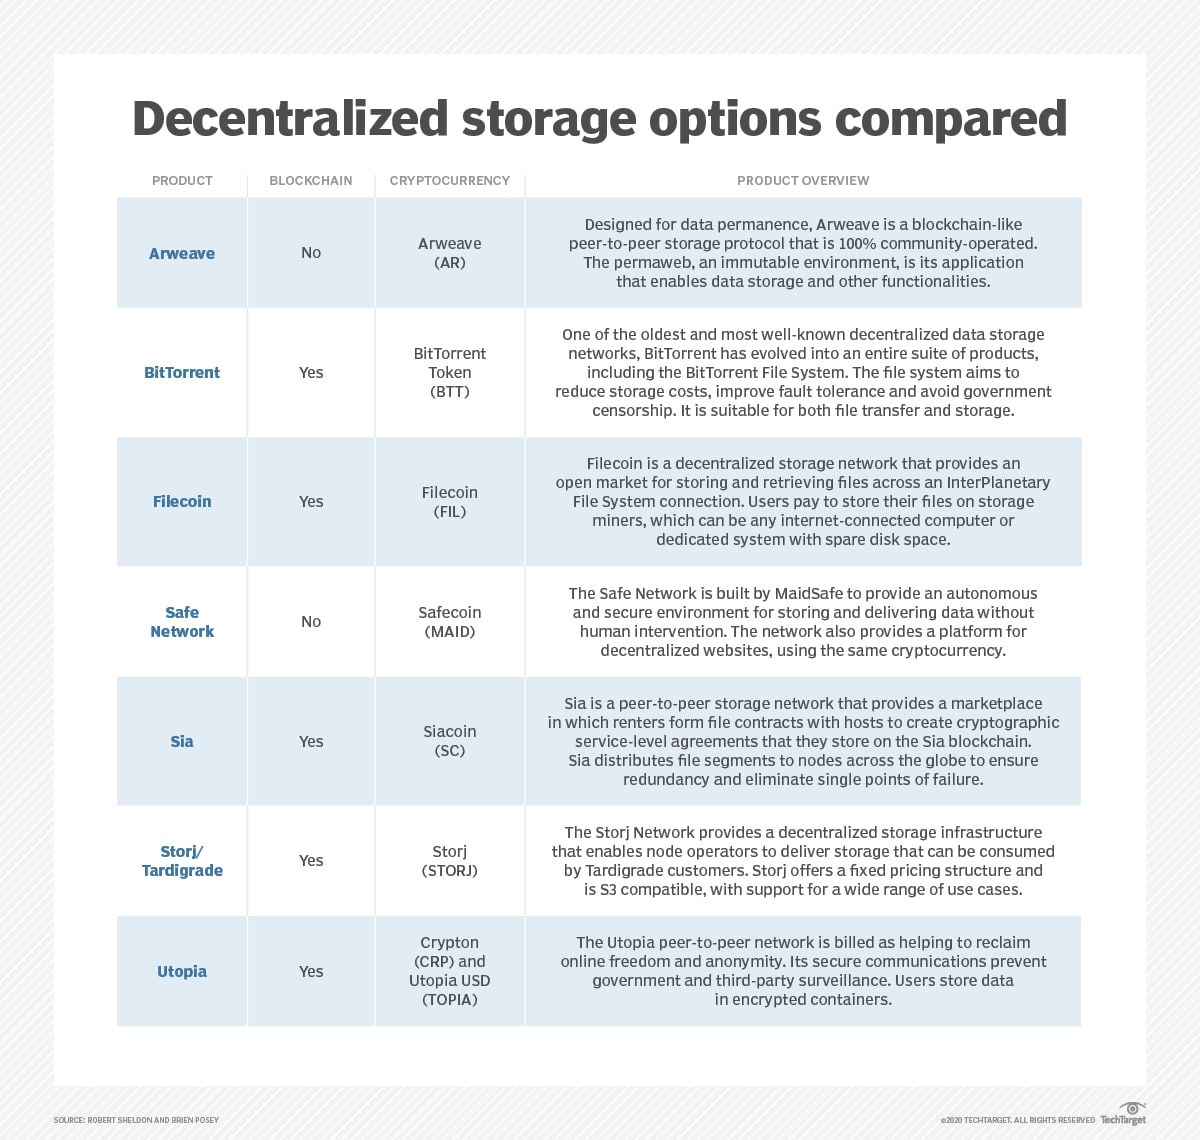
\includegraphics[width=\linewidth]{files}
  \caption{Comparison of distributed file stores}
  \label{fig:Files}
\end{figure}. 
\section{Risks \& Challenges?}
Classic DID/SSI risks fragmentations. 
In all DID scaling to a world where the user is managing potentially thousands of these critical cryptographic data files is daunting.
Abstracting the guts of this away to make the user simple, and only caring about right level of information, turns out to be huge problem that nobody has solved
It's not clear that users want this
In the case of web of trust like Slashtags it's a big piece of work for the users to rate off of their digital interactions with a trust metric.


